\let\negmedspace\undefined
\let\negthickspace\undefined
\documentclass[journal]{IEEEtran}
\usepackage[a5paper, margin=10mm, onecolumn]{geometry}
%\usepackage{lmodern} % Ensure lmodern is loaded for pdflatex
\usepackage{tfrupee} % Include tfrupee package

\setlength{\headheight}{1cm} % Set the height of the header box
\setlength{\headsep}{0mm}     % Set the distance between the header box and the top of the text

\usepackage{gvv-book}
%\usepackage{gvv}
\usepackage{cite}
\usepackage{amsmath,amssymb,amsfonts,amsthm}
\usepackage{algorithmic}
\usepackage{graphicx}
\usepackage{textcomp}
\usepackage{xcolor}
\usepackage{txfonts}
\usepackage{listings}
\usepackage{enumitem}
\usepackage{mathtools}
\usepackage{gensymb}
\usepackage{comment}
\usepackage[breaklinks=true]{hyperref}
\usepackage{tkz-euclide} 
\usepackage{listings}
\usepackage{gvv}                                        
\def\inputGnumericTable{}                                 
\usepackage[latin1]{inputenc}                                
\usepackage{color}                                            
\usepackage{array}                                            
\usepackage{longtable}                                       
\usepackage{calc}                                             
\usepackage{multirow}                                         
\usepackage{hhline}                                           
\usepackage{ifthen}                                           
\usepackage{lscape}
\begin{document}

\bibliographystyle{IEEEtran}

\title{4.6.7}
\author{EE25BTECH11019 - Darji Vivek M.}
{\let\newpage\relax\maketitle}

\renewcommand{\thefigure}{\theenumi}
\renewcommand{\thetable}{\theenumi}
\setlength{\intextsep}{10pt}
\numberwithin{figure}{enumi}
\renewcommand{\thetable}{\theenumi}

\textbf{Question}:\\
Find the equation of the line which passes through the point $(3,4,5)$ and is parallel to the vector $2\vec{i}+\vec{j}-3\vec{k}$.\\[4pt]
\hfill $\brak{12,2018}$

\solution \\[-2mm]
\textbf{Matrix Method:}\\
Let the point be
\begin{align}
\vec{A}=\myvec{3\\4\\5},
\end{align}
and the direction vector be
\begin{align}
\vec{d}=\myvec{2\\1\\-3}.
\end{align}

The general form of a line is
\begin{align}
\vec{r}=\vec{A}+\lambda\vec{d}.
\end{align}

Substituting values,
\begin{align}
\vec{r}=\myvec{3\\4\\5}+\lambda\myvec{2\\1\\-3}.
\end{align}

\begin{align}
\vec{r}=\boxed{\myvec{3+2\lambda\\4+\lambda\\5-3\lambda}}
\end{align}

Equation of line in symmetric form

\begin{align}
\frac{x-3}{2}=\frac{y-4}{1}=\frac{z-5}{-3}.
\end{align}

\begin{figure}[H]
\centering
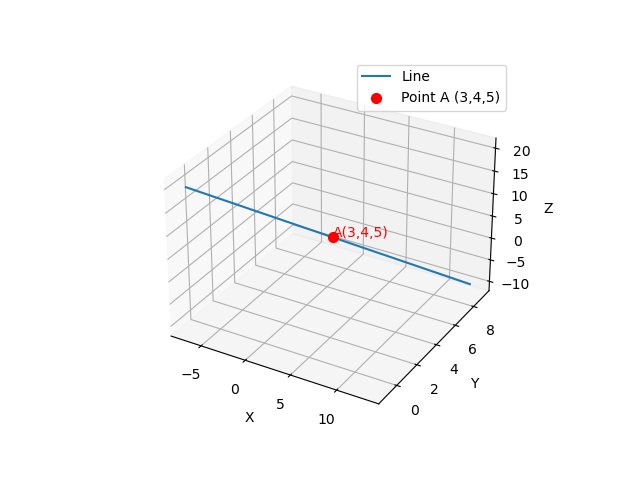
\includegraphics[width=0.75\columnwidth]{figs/7.png}
\caption{\centering Line through $\vec{A}$ parallel to $\vec{d}$}
\label{fig:line_eqn}
\end{figure}

\end{document}